%----------------------------------------------------------------------------------------
%	PACKAGES AND OTHER DOCUMENT CONFIGURATIONS
%----------------------------------------------------------------------------------------

\documentclass[18pt]{extarticle}

%%%%%%%%%%%%%%%%%%%%%%%%%%%%%%%%%%%%%%%%%
% Lachaise Assignment
% Structure Specification File
% Version 1.0 (26/6/2018)
%
% This template originates from:
% http://www.LaTeXTemplates.com
%
% Authors:
% Marion Lachaise & François Févotte
% Vel (vel@LaTeXTemplates.com)
%
% License:
% CC BY-NC-SA 3.0 (http://creativecommons.org/licenses/by-nc-sa/3.0/)
% 
%%%%%%%%%%%%%%%%%%%%%%%%%%%%%%%%%%%%%%%%%

%----------------------------------------------------------------------------------------
%	PACKAGES AND OTHER DOCUMENT CONFIGURATIONS
%----------------------------------------------------------------------------------------

\setlength{\parindent}{0em}
\setlength{\parskip}{.5em}

\usepackage{amsmath,amsfonts,stmaryrd,amssymb} % Math packages

\usepackage{enumerate} % Custom item numbers for enumerations

\usepackage[ruled]{algorithm2e} % Algorithms

\usepackage[framemethod=tikz]{mdframed} % Allows defining custom boxed/framed environments

\usepackage{dirtytalk}

\usepackage{listings} % File listings, with syntax highlighting
\lstset{
	basicstyle=\ttfamily, % Typeset listings in monospace font
}

\usepackage{hyperref}
\hypersetup{
    colorlinks=true,
    linkcolor=blue,
    filecolor=magenta,      
    urlcolor=cyan,
}


%----------------------------------------------------------------------------------------
%	DOCUMENT MARGINS
%----------------------------------------------------------------------------------------

\usepackage{geometry} % Required for adjusting page dimensions and margins

\geometry{
	paper=a4paper, % Paper size, change to letterpaper for US letter size
	top=2.5cm, % Top margin
	bottom=3cm, % Bottom margin
	left=2.5cm, % Left margin
	right=2.5cm, % Right margin
	headheight=14pt, % Header height
	footskip=1.5cm, % Space from the bottom margin to the baseline of the footer
	headsep=1.2cm, % Space from the top margin to the baseline of the header
	%showframe, % Uncomment to show how the type block is set on the page
}

%----------------------------------------------------------------------------------------
%	FONTS
%----------------------------------------------------------------------------------------

\usepackage[utf8]{inputenc} % Required for inputting international characters
\usepackage[T1]{fontenc} % Output font encoding for international characters

\usepackage{XCharter} % Use the XCharter fonts

%----------------------------------------------------------------------------------------
%	COMMAND LINE ENVIRONMENT
%----------------------------------------------------------------------------------------

% Usage:
% \begin{commandline}
%	\begin{verbatim}
%		$ ls
%		
%		Applications	Desktop	...
%	\end{verbatim}
% \end{commandline}

\mdfdefinestyle{commandline}{
	leftmargin=10pt,
	rightmargin=10pt,
	innerleftmargin=15pt,
	middlelinecolor=black!50!white,
	middlelinewidth=2pt,
	frametitlerule=false,
	backgroundcolor=black!5!white,
	frametitle={Command Line},
	frametitlefont={\normalfont\sffamily\color{white}\hspace{-1em}},
	frametitlebackgroundcolor=black!50!white,
	nobreak,
	singleextra={%
    }
}

% Define a custom environment for command-line snapshots
\newenvironment{commandline}{
	\medskip
	\begin{mdframed}[style=commandline]
}{
	\end{mdframed}
	\medskip
}

%----------------------------------------------------------------------------------------
%	FILE CONTENTS ENVIRONMENT
%----------------------------------------------------------------------------------------

% Usage:
% \begin{file}[optional filename, defaults to "File"]
%	File contents, for example, with a listings environment
% \end{file}

\mdfdefinestyle{file}{
	innertopmargin=1.6\baselineskip,
	innerbottommargin=0.8\baselineskip,
	topline=false, bottomline=false,
	leftline=false, rightline=false,
    leftmargin=0cm,rightmargin=0cm,
	singleextra={%
		\draw[fill=black!10!white](P)++(0,-1.2em)rectangle(P-|O);
		\node[anchor=north west]
		at(P-|O){\ttfamily\mdfilename};
		%
		\def\l{3em}
		\draw(O-|P)++(-\l,0)--++(\l,\l)--(P)--(P-|O)--(O)--cycle;
		\draw(O-|P)++(-\l,0)--++(0,\l)--++(\l,0);
	},
	firstextra={%
		\draw[fill=black!10!white](P)++(0,-1.2em)rectangle(P-|O);
		\node[anchor=north west]
		at(P-|O){\ttfamily\mdfilename};
		%
	},
    middleextra={%
    },
    secondextra={%
		\def\l{3em}
		\draw(O-|P)++(-\l,0)--++(\l,\l)--(P)--(P-|O)--(O)--cycle;
		\draw(O-|P)++(-\l,0)--++(0,\l)--++(\l,0);
    },
    nobreak,
}

% Define a custom environment for file contents
\newenvironment{file}[1][File]{ % Set the default filename to "File"
	\medskip
	\newcommand{\mdfilename}{#1}
	\begin{mdframed}[style=file]
}{
	\end{mdframed}
	\medskip
}

%----------------------------------------------------------------------------------------
%	NUMBERED QUESTIONS ENVIRONMENT
%----------------------------------------------------------------------------------------

% Usage:
% \begin{question}[optional title]
%	Question contents
% \end{question}

\mdfdefinestyle{question}{
	innertopmargin=1.2\baselineskip,
	innerbottommargin=0.8\baselineskip,
	roundcorner=5pt,
	singleextra={%
		\draw(P-|O)node[xshift=1em,anchor=west,fill=white,draw,rounded corners=5pt]{%
		Άσκηση \theQuestion\questionTitle};
	},
	firstextra={%
		\draw(P-|O)node[xshift=1em,anchor=west,fill=white,draw,rounded corners=5pt]{%
		Άσκηση \theQuestion\questionTitle};
	},
}

\newcounter{Question} % Stores the current question number that gets iterated with each new question

% Define a custom environment for numbered questions
\newenvironment{question}[1][\unskip]{
	\bigskip
	\stepcounter{Question}
	\newcommand{\questionTitle}{~#1}
	\begin{mdframed}[style=question]
}{
	\end{mdframed}
	\medskip
}

%----------------------------------------------------------------------------------------
%	WARNING TEXT ENVIRONMENT
%----------------------------------------------------------------------------------------

% Usage:
% \begin{warn}[optional title, defaults to "Warning:"]
%	Contents
% \end{warn}

\mdfdefinestyle{warning}{
	topline=false, bottomline=false,
	leftline=false, rightline=false,
	nobreak,
	singleextra={%
		\draw(P-|O)++(-0.5em,0)node(tmp1){};
		\draw(P-|O)++(0.5em,0)node(tmp2){};
		\fill[black,rotate around={45:(P-|O)}](tmp1)rectangle(tmp2);
		\node at(P-|O){\color{white}\scriptsize\bf !};
		\draw[very thick](P-|O)++(0,-1em)--(O);%--(O-|P);
	}
}

% Define a custom environment for warning text
\newenvironment{warn}[1][Warning:]{ % Set the default warning to "Warning:"
	\medskip
	\begin{mdframed}[style=warning]
		\noindent{\textbf{#1}}
}{
	\end{mdframed}
}

%----------------------------------------------------------------------------------------
%	INFORMATION ENVIRONMENT
%----------------------------------------------------------------------------------------

% Usage:
% \begin{info}[optional title, defaults to "Info:"]
% 	contents
% 	\end{info}

\mdfdefinestyle{info}{%
	topline=false, bottomline=false,
	leftline=false, rightline=false,
	nobreak,
	singleextra={%
		\fill[black](P-|O)circle[radius=0.4em];
		\node at(P-|O){\color{white}\scriptsize\bf i};
		\draw[very thick](P-|O)++(0,-0.8em)--(O);%--(O-|P);
	}
}

% Define a custom environment for information
\newenvironment{info}[1][Info:]{ % Set the default title to "Info:"
	\medskip
	\begin{mdframed}[style=info]
		\noindent{\textbf{#1}}
}{
	\end{mdframed}
}

\newcommand{\src}[1]{{\texttt{#1}}}

 % Include the file specifying the document structure and custom commands

%----------------------------------------------------------------------------------------
%	ASSIGNMENT INFORMATION
%----------------------------------------------------------------------------------------

\title{Εργασία Ανάπτυξης Αρθρώματος Πυρήνα (Kernel Module) \\Λειτουργικά Συστήματα (ECE ΓΚ702)} % Title of the assignment

% \author{\footnotesize Χρήστος Φείδας\\ \footnotesize \src{fidas@upatras.gr} \and \footnotesize Ευάγγελος Λάμπρου\\ \footnotesize \src{e.lamprou@upnet.gr}} % Author name and email address

\date{Πανεπιστήμιο Πατρών --- \the\year{}} % University, school and/or department name(s) and a date

\usepackage{fancyhdr}

%----------------------------------------------------------------------------------------

\begin{document}

\pagestyle{fancy}
%... then configure it.
\fancyhf{} % sets both header and footer to nothing
\renewcommand{\headrulewidth}{0pt}
\fancyhead{} % clear all header fields
\fancyfoot{} % clear all footer fields
\fancyfoot[L]{Χρήστος Φείδας, Ευάγγελος Λάμπρου}
\fancyfoot[R]{\thepage}

\maketitle

%----------------------------------------------------------------------------------------
%	INTRODUCTION
%----------------------------------------------------------------------------------------

\section{Εισαγωγή}

Η εργασία αυτή κάνει μία εισαγωγή στη συγγραφή απλών αρθρωμάτων πυρήνα (kernel modules) 
για το λειτουργικό σύστημα Linux.

Μία λεπτομερή εισαγωγή για το Linux μπορείτε να βρείτε \href{https://linux-kernel-labs.github.io/refs/heads/master/lectures/intro.html}{εδώ}.

\subsection{Ο πηγαίος κώδικας του Linux kernel.}

Ο πηγαίος κώδικας του Linux kernel είναι διαθέσιμος ελεύθερα. 
Κάποιος μπορεί να κατεβάσει τον κώδικα, να τον επεξεργαστεί και να δημιουργήσει δικές του εκδόσεις του Linux kernel.
Στα πλαίσια των εργασιών θα ζητηθεί να αναζητήσετε ορισμούς μέσα από τον πηγαίο κώδικα.

Τρόποι εξευρεύνησης του πηγαίου κώδικα είναι:

\begin{itemize}
    \item Λήψη του κώδικα από το \href{https://kernel.org/}{kernel.org} και χρήση του αγαπημένου σας editor (Visual Studio Code, Vim, Emacs ...) για αναζήτηση σε αυτόν.
    \item Χρήση της ιστοσελίδας \href{https://elixir.bootlin.com/linux/latest/source}{elixir.bootlin.com} (προτείνεται)
\end{itemize}

\subsection{Τί είναι ένα Kernel Module;}

Ο πυρήνας (kernel) των Linux είναι μονολιθικός, πράγμα που σημαίνει πως αν κάποιος ήθελε να 
προσθέσει νέα λειτουργικότητα σε αυτόν θα έπρεπε να επεξεργαστεί τον πηγαίο κώδικα, 
να τον επαναμεταγλωτίσει (recompile) και να κάνει επανεκκίνηση το σύστημά του ώστε να δει τις αλλαγές του.

Αυτή η διαδικασία προφανώς είναι κουραστική και περίπλοκη. Έτσι, ο πυρήνας Linux 
υποστηρίζει modules (αρθρώματα) τα οποία φορτώνονται στον ήδη υπάρχοντα πυρήνα κατά τη διάρκεια εκτέλεσής του
και μπορούν να είναι οδηγοί συσκευής (device drivers), κάποιο σύστημα αρχέιων (file system), πρωτόκολλο δικτύωσης
(network protocol) κ.α.

\begin{figure}[htpb]
    \centering
    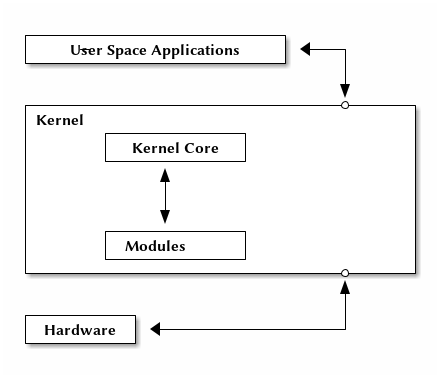
\includegraphics[width=0.6\textwidth]{assets/module.png}
    \caption{Όταν ένα kernel module φορτώνεται είναι πλέον μέρος του πυρήνα.}
    \label{fig:module}
\end{figure}

\subsection{Προετοιμασία περιβάλλοντος ανάπτυξης.}

Ένα kernel module έχει άμεση πρόσβαση στο υλικό του συστήματος.
Αυτό σημαίνει πως υπάρχει η δυνατότητα να φέρει το σύστημα σε κατάσταση που χρειάζεται η επανεκκίνσή του.
Για αυτό το λόγο προτείνεται να δουλέψετε σε κάποιο εικονικό μηχάνημα (virtual machine) ώστε να αποφύγετε το ρίσκο βλάβης στο σύστημά σας.

Για να έχετε ένα εικονονικό μηχάνημα μπορείτε να χρησιμοποιήσετε το δωρεάν λογισμικό \href{https://www.virtualbox.org/}{Virtual Box}
Από εκεί, μπορείτε να δημιουργήσετε ένα εικονικό μηχάνημα χρησιμοποιώντας οποιαδήποτε διανομή των Linux επιθυμείτε.  
Διαφοροποιήσεις μεταξύ διανομών θα υπάρχουν μόνο στη διαδικασία απόκτησης των απαραίτητων πακέτων για την ανάπτυξη του κώδικα του module.

Για να είναι η ανάπτυξη του κώδικα γρηγορότερη, χρήσιμο θα ήταν να χρησιμοποιήσετε τη δυνατότητα "shared folder" του Virtual Box,
έτσι ώστε να γίνεται η συγγραφή του κώδικα στο κανονικό σας σύστημα και έπειτα η μεταγλώττιση και φόρτωση των modules στο εικονικό μηχάνημα.
Οδηγίες για αυτό μπορείτε να βρείτε \href{https://www.virtualbox.org/manual/ch04.html#sharedfolders}{εδώ} και \href{https://carleton.ca/scs/tech-support/troubleshooting-guides/creating-a-shared-folder-in-virtualbox/}{εδώ}.
Εναλλακτικά μπορείτε να κάνετε ακόμα και τη συγγραφή του κώδικα στο εικονικό σας μηχάνημα εγκαθιστώντας σε αυτό κάποιον επεξεργαστή κειμένου.

\subsubsection{Απαραίτητα Πακέτα}

Θα χρειαστεί να υπάρχουν στο σύστημά σας ορισμένα πακέτα και τα σχετικά header files:

Για διανομές βασισμένες στα Debian:

\begin{commandline}
	\begin{verbatim}
$ sudo apt-get update

$ sudo apt-get install build-essential kmod
$ sudo apt-get install linux-headers-`uname -r`
	\end{verbatim}
\end{commandline}


Για διανομές βασισμένες στα Arch:

\begin{commandline}
	\begin{verbatim}
$ sudo pacman -S gcc kmod
$ sudo pacman -S linux-headers
	\end{verbatim}
\end{commandline}


\begin{warn}[Προσοχή]
Φροντίστε να έχετε κατεβάσει τους κατάλληλους linux-headers για την έκδοση του Linux kernel που τρέχει στο σύστημά σας.
Μπορείτε να τη βρείτε με την εντολή \src{uname -r}.
\end{warn}

\subsection{Ένα Παράδειγμα}

Για αρχή, στο σύστημά σας ανοίξτε ένα τερματικό (terminal).
Εκτελέστε την εντολή \src{su} και πληκτρολογήστε το root password ώστε να εκτελέσετε όλες τις υπόλοιπες εντολές ως διαχειριστής (root). 
Πολλές από τις εντολές διαχείρισης modules πρέπει να εκτελούνται με δικαιώματα root.

Μπορείτε να δείτε τα modules που είναι τώρα φορτωμένα στο σύστημά σας με την
εντολή \src{sudo lsmod}.

Φτιάξτε ένα φάκελο.
Εκεί θα βρίσκονται όλα τα αρχεία που θα αφορούν το module που θα φτιάξουμε.

\begin{commandline}
	\begin{verbatim}
$ mkdir ~/hello-world
$ cd ~/hello-world
	\end{verbatim}
\end{commandline}

\subsubsection{Kernel Module - Hello World}

Αποθηκεύστε τον παρακάτω κώδικα σε ένα αρχείο με όνομα \src{hello.c}.

\begin{file}[hello.c]
    \lstinputlisting[language=C]{../src/hello/hello.c}
\end{file}

Ο κώδικας που βρίσκεται στη συνάρτηση \src{my\_init} θα εκτελεστεί όταν φορτώσουμε το module μας. 
Εδώ γίνονται τυχόν αρχικοποιήσεις πόρων που θα χρειαστεί το module. 
Επιστρέφει έναν ακέραιο ανάλογα με τον αν ήταν επιτυχής ή όχι η αρχικοποίηση του module.
Ο κώδικας που βρίσκεται στη συνάρτηση \src{my\_exit} θα εκτελεστεί όταν αποφορτώσουμε το module μας. 
Εδώ θα πρέπει το module μας να επιστρέψει πίσω στο σύστημα τυχόν πόρους που έχει δεσμεύσει.

Οι μακροεντολές (macros) \src{module\_init} και \src{module\_exit} ορίζουν τις συναρτήσεις μας ως συναρτήσεις "εκίννησης" και "εξόδου" για το τελικό kernel object.

Οι μακροεντολές \src{MODULE\_DESCRIPTION}, \src{MODULE\_AUTHOR} και \src{MODULE\_LICENSE} ορίζουν metadata για το module μας.

Παρατηρήστε τη χρήση της συνάρτησης \src{printk} έναντι κάτι όπως \src{printf}.
Όταν αναπτύσετε κώδικα σε kernel space, δεν έχετε διαθέσιμη τη βασική βιβλιοθήκη της C. 
Έχετε διαθέσιμα μόνο σύμβολα τα οποία έχουν οριστεί από τον πυρήνα.
Για να δείτε τα σύμβολα που είναι ορισμένα από τον πυρήνα στο σύστημά σας εκτελέστε την εντολή \src{cat /proc/kallsyms}.

Αποθηκεύστε τον παρακάτω κώδικα σε ένα αρχείο με όνομα \src{Makefile}.

\begin{file}[Makefile]
    \footnotesize \lstinputlisting[language=C, tabsize=2]{../src/hello/Makefile}
\end{file}

Αυτό το αρχείο ορίζει τις εντολές οι οποίες θα εκτελεστούν για να μεταγλωτιστεί 
το module που φτιάχνουμε.

\begin{info}[Σημείωση:]
Στο αρχείο \src{Makefile} (και σε όλα τα \src{makefiles} γενικότερα) πρέπει κάτω από το όνομα του κάθε κανόνα (\src{all, clean}) να υπάρχει χαρακτήρας \src{<TAB>}.
Αυτό είναι παρόμοιο με τον τρόπο που η γλώσσα Python χειρίζεται τις block δομές της.
\end{info}

Για να μεταγλωτίσετε το module, στον φάκελο που έχετε όλα τα αρχείο εκτελέστε την εντολή \src{make}.
Για να σβήσετε τα αρχεία που δημιουργούνται από τη μεταγλώτισση μπορείτε να χρησιμοποιήσετε την εντολή \src{make clean}.

Ο φάκελός σας πρέπει τώρα να περιέχει τα παρακάτω αρχεία:

\begin{commandline}
\begin{verbatim}
$ ls hello-world

../hello-world
├── hello.c
├── hello.ko
├── hello.mod
├── hello.mod.c
├── hello.mod.o
├── hello.o
├── Makefile
├── modules.order
└── Module.symvers
\end{verbatim}
\end{commandline}


Από αυτά, το αρχείο \src{hello.ko} είναι το τελικό kernel object το οποίο και θα φορτώσουμε στον 
πυρήνα του συστήματός μας. 

Μπορείτε να δείτε μερικές πληροφορίες για το module με την εντολή: 
\begin{commandline}
\begin{verbatim}
$ modinfo hello.ko
\end{verbatim}
\end{commandline}

% Δοκιμάστε να τρέξετε την παρακάτω εντολή ώστε να επιβεβαιώσετε πως το module μας δεν είναι ακόμα φορτωμένο στον πυρήνα:
% 
% \begin{commandline}
% \begin{verbatim}
% $ sudo lsmod | grep hello
% \end{verbatim}
% \end{commandline}

Μπορούμε πλέον να \textbf{φορτώσουμε} το module στο σύστημά μας με την εντολή:

\begin{commandline}
\begin{verbatim}
$ sudo insmod hello.ko
\end{verbatim}
\end{commandline}

Τώρα θα δείτε το module μας στη λίστα με τα modules του συστήματος αν εκτελέσουμε:

\begin{commandline}
\begin{verbatim}
$ sudo lsmod | grep hello
\end{verbatim}
\end{commandline}

Για να \textbf{αφαιρέσουμε} το module μας εκτελούμε την εντολή:


\begin{commandline}
\begin{verbatim}
$ sudo rmmod hello
\end{verbatim}
\end{commandline}

Τώρα αν ελέγξουμε τα logs του συστήματος με την εντολή: 

\begin{commandline}
\begin{verbatim}
$ journalctl --since "10 minutes ago" | grep kernel
\end{verbatim}
\end{commandline}

Μπορούμε να δούμε τα μηνύματα που είχαμε προσθέσει στις 
συναρτήσεις \src{my\_init} και \src{my\_exit}

Το module μας δεν έχει δυνατότητα εκτύπωσης μυνημάτων σε γραφική κονσόλα (υπάρχει βέβαια δυνατότητα εξόδου σε κονσόλα τύπου tty). 
Για αυτό πρέπει να βλέπουμε τα μυνήματα από τα logs του συστήματος.

\section{Ασκήσεις}

\begin{question}
Τροποποιήστε το αρχικό module που φτιάξαμε ώστε να τυπώνει ένα διαφορετικό μήνυμα. \\
Ακολουθήστε την ίδια διαδικασία για την φόρτωση/εκφόρτωσή του.                                                                                                               

% Δοκιμάστε να γράψετε σε μία διεύθυνση που δεν σας ανήκει ή βάλτε στην συνάρτηση εκκίνησης του module ένα ατέρμονο loop.
% Θα παρατηρήσετε πως ο πυρήνας είναι ανθεκτικός σε μερικά σφάλματα τα οποία θα οδηγούσαν σε crash ένα πρόγραμμα που εκτελείται σε user space. 
\end{question}

\begin{info}[Σημείωση:]
Μήν βασιστείτε σε απλή αντιγραφή-επικόλληση του κώδικα.                                                                        
Προσπαθήστε να γράψετε μόνοι σας από την αρχή το πρόγραμμα γραμμή-γραμμή ώστε να γίνει κατανοητή η δομή του.                                 
\end{info}

\begin{question}
    Πηγαίνετε στον πηγαίο κώδικα του Linux kernel και διαβάστε τον ορισμό για το \src{task\_struct} (στο αρχείο \src{linux/include/linux/sched.h}.
Τί πληροφορίες αποθηκεύονται σε αυτή τη δομή; Τί αντιπροσωπεύει;

\begin{info}[Σημείωση:]
    Για μια λεπτομερή παρουσίαση της δομής \src{task\_struct} και του διαχειρισμού διεργασιών 
    στο Linux Kernel μπορείτε να βρείτε στο βιβλίο \href{https://www.doc-developpement-durable.org/file/Projets-informatiques/cours-&-manuels-informatiques/Linux/Linux\%20Kernel\%20Development,\%203rd\%20Edition.pdf}{Linux Kernel Development}
    (Κεφάλαιο 3).
\end{info}
\end{question}

\begin{question}
Γράψτε ένα module πυρήνα το οποίο Θα τυπώνει πληροφορίες για όλες τις υπάρχουσες διεργασίες όταν φορτώνεται.
Για να πάρουμε έναν δείκτη προς την διεργασία που εκτελείται αυτή τη στιγμή μπορούμε να χρησιμοποιήσουμε
το macro \src{current}. Μπορείτε να βρείτε τον ορισμό του macro αυτού μέσα στο αρχείο \src{linux/arch/x86/include/asm/current.h}.

Ξεκινήστε με τον παρακάτω κώδικα σαν βάση.

Κάντε τις κατάλληλες προσθήκες στη συνάρτηση \src{my\_proc\_init} (σημείο \src{TODO}) ώστε να τυπωθούν οι αντίστοιχες πληροφορίες για όλες τις διεργασίες του συστήματος. 

Για το πώς γίνεται αυτό κοιτάξτε στο αρχείο (\src{linux/include/linux/sched/signal.h} στο macro \src{for\_each\_process}).

\begin{file}[list-processes.c]
    \footnotesize \lstinputlisting[language=C, tabsize=2]{../src/list-proc/list-proc-basic.c}
\end{file}

\begin{info}[Σημείωση]
Θα πρέπει για το νέο module να φτιάξετε νέο φάκελο και εκεί
να τοποθετήσετε τον πηγαίο κώδικα (.c αρχείο) και το \src{Makefile} κάνοντας κατάλληλη αλλαγή σε αυτό. 
Η διαδικασία μεταγλώττισης θα είναι ίδια όπως με το πρώτο module που φτιάξατε.
\end{info}

\end{question}

\begin{question}
   Στην άσκηση αυτή σας ζητείται να φτιάξετε ένα kernel module το οποίο θα τυπώνει πληροφορίες για μία διεργασία και τις θυγατρικές τις διεργασίες.
   
   Ξεκινήστε δημιουργώντας ένα πρόγραμμα όπως το παρακάτω.

    \begin{file}[forking.c]
        \footnotesize \lstinputlisting[language=C, tabsize=2]{../src/show-children/main.c}
    \end{file}

    Μεταγλωτίστε και έπειτα εκτελέστε το πρόγραμμα με τις εντολές:

   \begin{commandline}
       \begin{verbatim}
   $ gcc forking.c -o forking
   $ ./forking
       \end{verbatim}
   \end{commandline}

    Αυτό το πρόγραμμα ανά \src{SLEEP\_TIME} δευτερόλεπτα εκτελεί την κλήση συστήματος (\href{https://man7.org/linux/man-pages/man2/syscalls.2.html}{system call}) \src{fork}.
    Ζητείται μέσα από το kernel που θα γράψετε να βρείτε τη δομή \src{task\_struct} που αντιστοιχεί 
    σε αυτή τη διεργασία με βάση το \src{PID} της και έπειτα να τυπώσετε το \src{PID} καθεμίας από τις διεργασίες παιδιά της.

    \begin{center}
        \centering
        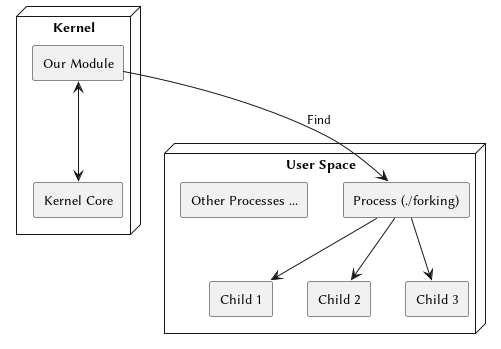
\includegraphics[width=0.8\textwidth]{assets/process.png}
    \end{center}

    Το πρόγραμμα \src{forking} θα το αφήσετε να τρέχει. Σε άλλο τερματικό θα χρειαστεί να μεταγλωττίσετε και να φορτώσετε το module σας.

    Στο αρχείο \src{list-children.c} βρίσκεται ο σκελετός με βάση τον οποίο θα προσθέσετε τη ζητούμενη λειτουργικότητα.
    Συμπληρώστε τον κώδικά σας στο σημείο \src{TODO}.

    Θα πρέπει να εκτελέσετε το πρόγραμμά σας, να θέσετε το κατάλληλο PID στο module σας για να βρει τη διεργασία, να το μεταγλωττίσετε και έπειτα να το φορτώσετε.

\begin{warn}[Προσοχή]
    Αν κάνετε επανεκκίνηση τη διεργασία σας, πιθανότατα θα έχει ένα νέο, διαφορετικό \src{PID}.
    Έτσι, για να τυπώσετε πληροφορίες για τα παίδια της από το module σας θα πρέπει να εκφορτώσετε το module σας, να αλλάξετε το \src{PID} το οποίο θα αναζητήσει, 
    να το επαναμεταγλωτίσετε και να το επαναφορτώσετε.
\end{warn}

    Για να έχετε πρόσβαση στις διεργασίες-παιδιά μιας διεργασίας, χρησιμοποιήστε το μέλος \src{children} του \src{task\_struct}.
    Αυτό είναι μία δομή διπλά διασυνδεδεμένης λίστας στους κόμβους της οποίας βρίσκονται δομές \src{task\_struct *}.
    Στο Linux Kernel υπάρχουν διάφορα βοηθητικά macros για το χειρισμό λιστών.

    \begin{enumerate}
        \item Εντοπίστε τα πεδία \src{children} και \src{sibling} στην δομή \src{task\_struct} (στον πηγαίο κώδικα του Linux Kernel), τί αντιπροσωπεύει το καθένα;
        \item Διαβάστε τον τρόπο χρήσης του βοηθητικού macro \src{list\_for\_each\_entry}\\
            (στο αρχείο \src{linux/tools/include/linux/list.h})
        \item Προσθέστε στο σκελετό της άσκησης τον κατάλληλο κώδικα ώστε να τυπώνεται το PID κάθε διεργασίας παιδί της αρχικής σας διεργασίας, τί παρατηρείτε;    
    \end{enumerate}
    
\end{question}
    
\newpage

\section*{Περισσότερες Πηγές}

\begin{itemize}
    \item \href{https://www.doc-developpement-durable.org/file/Projets-informatiques/cours-&-manuels-informatiques/Linux/Linux\%20Kernel\%20Development,\%203rd\%20Edition.pdf}{Linux Kernel Development}
    \item \href{https://sysprog21.github.io/lkmpg/}{Linux Kernel Module Programming Guide}
    \item \href{https://lwn.net/Kernel/LDD3/}{Linux Device Drivers}
    \item Operating System Concepts 9th Edition - Silbershatz, Galvin, Gagne (ch. 18)
\end{itemize}

\end{document}
